%!TEX root = ../crimson_throne_book_main.tex


\begin{titlepage}
    \begin{tikzpicture}[remember picture, overlay]
		\fill[yellow!10] (current page.north west) rectangle (current page.south east);

% 		\node[above left] at  ($(current page.south east) + (0.5 cm, -0.5cm) $) {\includegraphics[width=1.05\pagewidth,trim={0 0 1.75cm 0},clip]{C:/privat/rpg/crimson_throne_book/latex/images/titlepage.jpg}};
		\node[above left] at  ($(current page.south east) + (0.5 cm, -0.5cm) $) {\includegraphics[width=1.05\pagewidth,trim={0 0 1.75cm 0},clip]{images/titlepage.jpg}};

		\fill[white] (current page.north west) rectangle ($(current page.north east) - (0cm, 6cm) $);
		\fill[orange, opacity=0.1] (current page.north west) rectangle ($(current page.north east) - (0cm, 6cm) $);


		\fill[white, opacity=0.6] (current page.north west) rectangle ($(current page.south west) + (2cm, 0cm) $);

        \node[font=\bfseries\setmainfont{Immortal}\fontsize{1cm}{2cm}\selectfont, rotate=90, right] at  ($(current page.south west) + (1cm, 0.25cm) $){Curse of the Crimson Throne};

		\node[align=right, below left, font=\bfseries\setmainfont{Immortal}\fontsize{0.75cm}{0.8cm}\selectfont] at($(current page.north east) - (0.5cm, 0.5cm) $) {Mr Veerge's Journal\\[2.5em] The adventures\\ of the\\ Pseudo Dragons };
    \end{tikzpicture}
\end{titlepage}